\documentclass[12pt, a4paper]{article}

% --- Paquetes básicos ---
\usepackage[utf8]{inputenc}
\usepackage[spanish]{babel}
\usepackage[margin=2.5cm]{geometry}
\usepackage{graphicx}
\usepackage{float}
\usepackage{amsmath, amssymb}
\usepackage{fancyhdr}

% --- Configuración del Título ---
\title{Bloque 2: Simulación de Carga de Trabajo y Monitorización}
\author{Juan Reche Aguilar}
\date{\today}

% --- Configuración de Encabezados ---
\pagestyle{fancy}
\fancyhf{}
\rhead{Ingeniería de Servidores}
\lhead{Juan Reche Aguilar}
\cfoot{\thepage}

\begin{document}

\maketitle

\tableofcontents
\newpage

\section{ Ejercicio 4.1.1. Stress + Top. }

\begin{figure}[H]
    \centering

    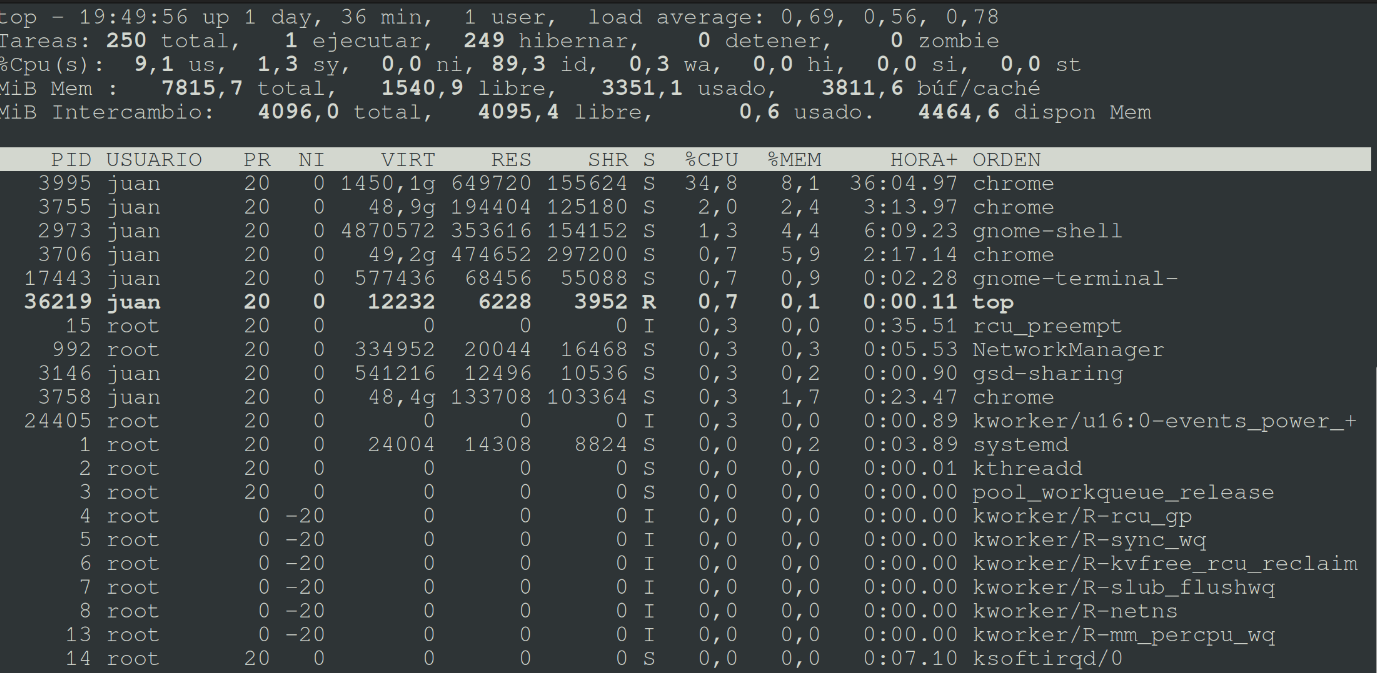
\includegraphics[width=1\textwidth]{../../capturas4/seccion1/top_sin_stress.png}

    \caption{Ejecucion de top antes de simular carga de trabajo.}

\end{figure}

\begin{figure}[H]
    \centering

    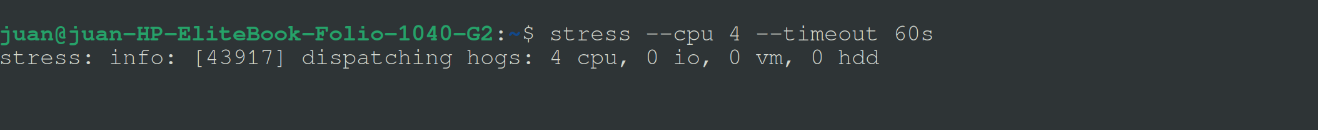
\includegraphics[width=1\textwidth]{../../capturas4/seccion1/stress.png}

    \caption{Ejecucion del programa stress.}

\end{figure}

\begin{figure}[H]
    \centering

    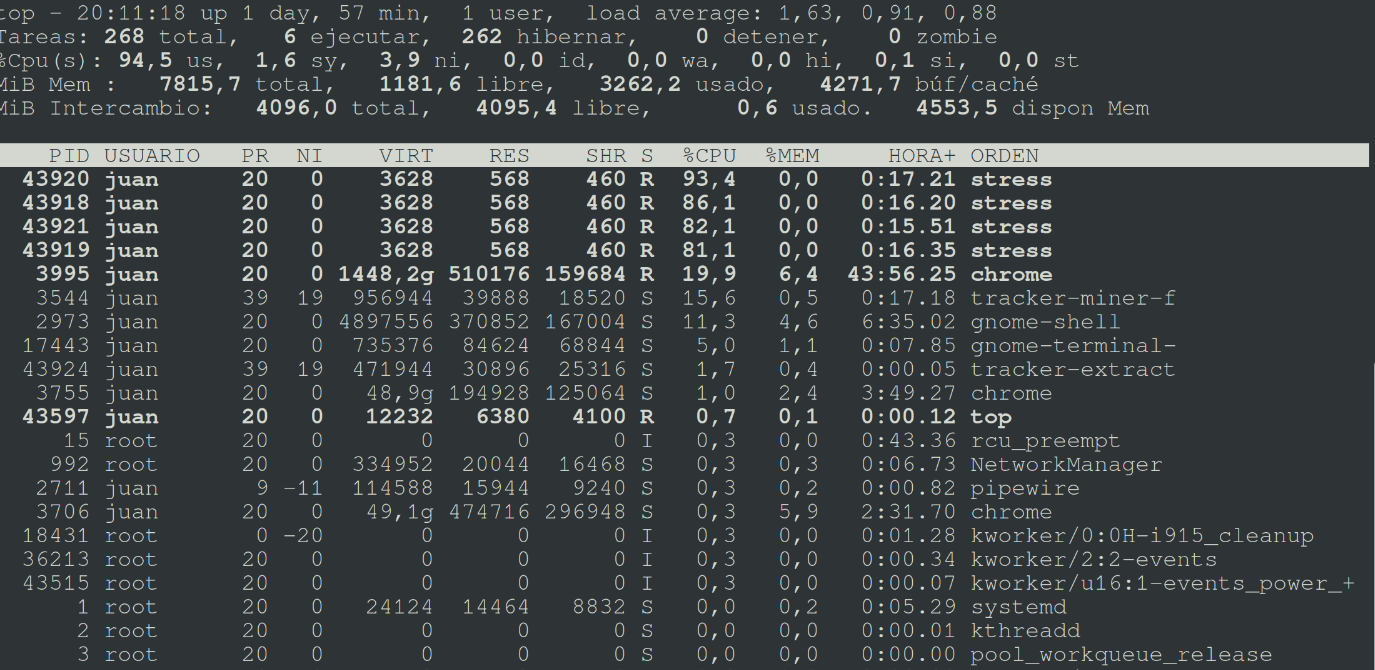
\includegraphics[width=1\textwidth]{../../capturas4/seccion1/top_stress.png}

    \caption{Ejecucion de top durante la simulacion de carga de trabajo.}

\end{figure}

En un primer monento, se ha ejecutado el programa \texttt{top} para observar el estado del sistema 
antes de simular la carga de trabajo, podemos ver múltiples procesos en ejecución como por ejemplo chrome. 
Posteriormente, se ha ejecutado el programa \texttt{stress} para generar una carga de trabajo en el sistema. 
Finalmente, se ha vuelto a ejecutar \texttt{top} durante la simulación de carga de trabajo para observar cómo 
afecta al sistema, se puede ver un aumento en el uso de CPU y los cuatro procesos generados.

\end{document}